\section{Overview}

%\cite{belair}, SkyPilot\footnote{It is a company}, BearCom, and so
%on.
\subsection{Atmospheric dispersion modeling}
In order to simulate the air pollution, we find out a well known air dispersion 
model which is a partial differential equation based on the law of 
conservation of mass. The solution of this differential equation can give us 
a function coordination to calculate the mass concentration of every point in 
the space.  

%\cite{fixed} shows an example of the most known one, video
%surveillance system. $\omega$

\subsection{Scenario}
In the atmospheric dispersion model we assumed that the wind speed and direction
is already known. However, in more realize case this assumption is over ideal 
assumption. Hence, based on this model, we relax the restriction of information 
about wind and make the wind speed as a random variable with some resonable 
distribution. Then we set up the  pollutant concentration sensor which distributed
uniformly as the cellular base station. 

\subsection{Algorithm}
When the pollutant is spreading in the space, the sensor start sensing the 
pollutant concentration nearby itself, and re-transmitted the data back to the 
cluster head. After that, server will reconstruct the pollutant distribution map 
which can point out that some certain area suffer from the pollutant seriously.
On the other hand, our wireless sensor might be restricted by the channel capacity,
and not all of the sensor could transmit data to cluster head. According to the 
scenario, we can derive a optimization problem with the entropy as the objective
function, in order to solve this problem, we apply the cross entropy algorithm
to find the approximate solution.  
 
\subsection{Performance analysis}
After the approximate solution is derived, we can conclude that the mean square
error of reconstruction map will be bounded through theoretical result of information
theory. Meanwhile, in order to validate the theoretical bound, we keep the air 
dispersion modeling result as the theoretical value and the reconstruction value 
as the measure value, and we can calculate the the mean square error from these two
part of result. Considering the mean square result, we can verify if the experiment 
result is consist with the theoretical bound. 



%\begin{figure}
%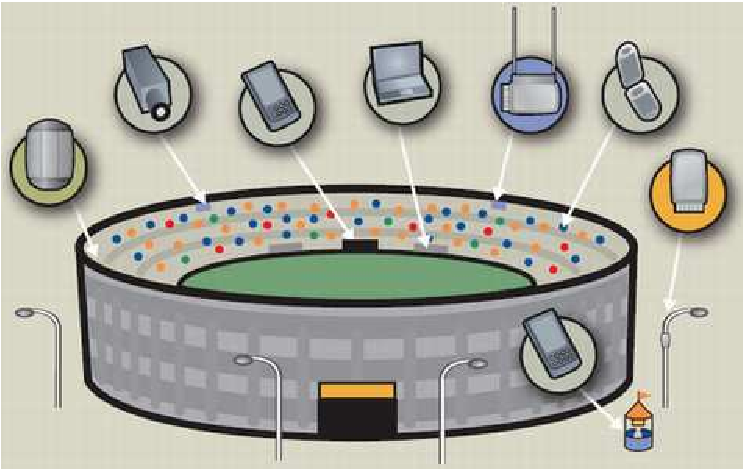
\includegraphics[scale=0.7 ,angle=0]{gym}
%\caption{A WMN video streaming topology in the gym}
%\label{gym}
%\end{figure}

%\begin{figure}
%\includegraphics[scale=0.8 ,angle=0,bb=140 300 470 520, clip]{video}
%\caption{The surveillance system over WMNs} \label{video}
%\end{figure}


